\documentclass[12pt]{article}
\usepackage[top=1in, bottom=1in, left=1in, right=1in]{geometry}

\usepackage{setspace}
\onehalfspacing

\usepackage[hang,flushmargin]{footmisc} 
% 'hang' flushes the footnote marker to the left,  'flushmargin'  flushes the text as well.

\def\baselinestretch{1}
\setlength{\parindent}{0mm} \setlength{\parskip}{0.8em}

\newlength{\up}
\setlength{\up}{-4mm}

\newlength{\hup}
\setlength{\hup}{-2mm}

\usepackage{amssymb}
%% The amsthm package provides extended theorem environments
\usepackage{amsthm}
\usepackage{epsfig}
\usepackage{times}
\renewcommand{\ttdefault}{cmtt}
\usepackage{amsmath}
\usepackage{graphicx} % for graphics files

% Draw figures yourself
\usepackage{tikz} 

% The float package HAS to load before hyperref
\usepackage{float} % for psuedocode formatting
\usepackage{xspace}

% from Denovo Methods Manual
\usepackage{mathrsfs}
\usepackage[mathcal]{euscript}
\usepackage{color}
\usepackage{array}

\usepackage[pdftex]{hyperref}
\usepackage{cancel}

\newcommand{\nth}{n\ensuremath{^{\text{th}}} }
\newcommand{\ve}[1]{\ensuremath{\mathbf{#1}}}
\newcommand{\Macro}{\ensuremath{\Sigma}}
\newcommand{\vOmega}{\ensuremath{\hat{\Omega}}}

\begin{document}
\begin{center}
{\bf NE 155, Classes 15-19, S15 \\
TE and DE \\ February 25 -- March 6, 2015}
\end{center}

\setlength{\unitlength}{1in}
\begin{picture}(6,.1) 
\put(0,0) {\line(1,0){6.25}}         
\end{picture}

%-------------------------------------------------------------
\section*{Transport Equation}

Largely from Lewis and Miller Chp.\ 1 \cite{Lewis1993} and Duderstadt and Hamilton Chp.\ 4 \cite{Duderstadt1976}. Note: Duderstadt and Martin \cite{Duderstadt1979} is a very good general reference. It goes through all of this same stuff, but from a slightly more generic point of view (since this applies to \underline{any} collection of neutral particles).

\subsection*{Definitions}

\begin{figure}[h!]
    \begin{center}
    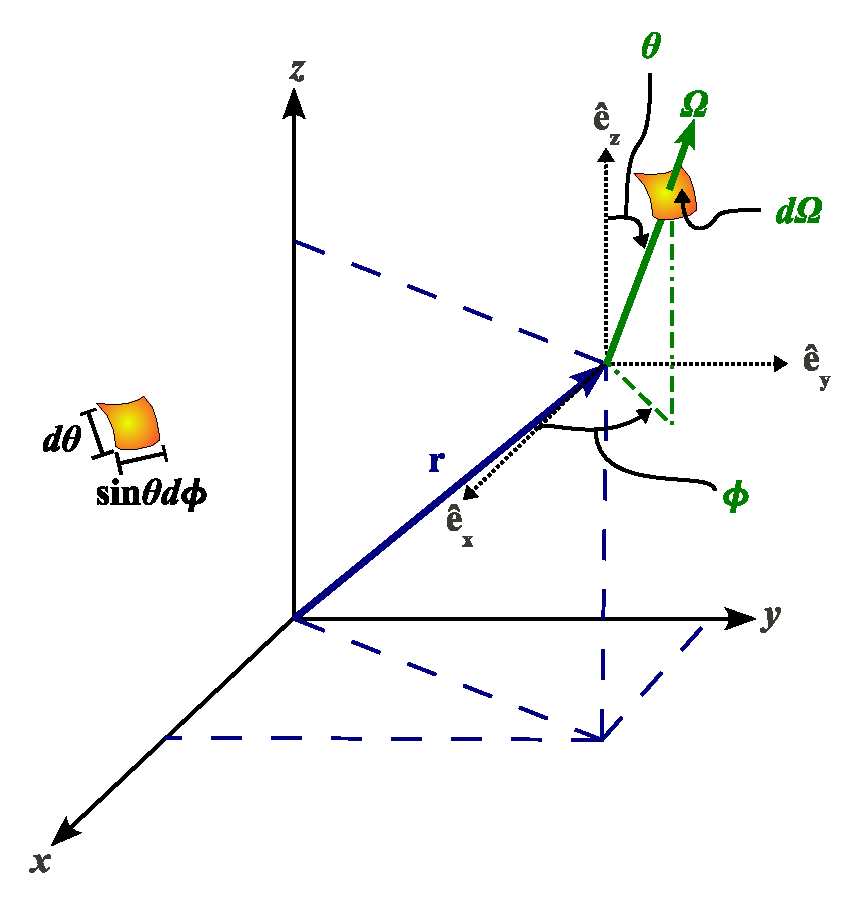
\includegraphics[keepaspectratio, width = 2.7 in]{phase_space}
    \end{center}
    \caption{Schematic of Phase Space}
    \label{fig:phase_space}
\end{figure}

Spatial logistics
\begin{itemize}
\item $d\vec{r} = d^3r$ = ordinary volume = $r^2 sin(\theta) d\theta d\varphi dr$
%
\item $v$ = speed (scaler)
\item $\vec{v}$ = velocity (vector)
\item $d\vec{v} = d^3v$ = velocity volume = $v^2 sin(\theta')d\theta' d\varphi' dr$
\item $v = \sqrt{(2E)/m}$ where $m$ is the rest mass of the particle. Thus, we can relate energy and speed.

\item $\vOmega$: unit directional vector in velocity space, $\vec{v} = v\vOmega$
\item $d\vOmega = sin(\theta')d\theta' d\varphi' =  d^2\Omega$
%\item thus $d\vec{v} = v^2 dv d\vOmega$
\end{itemize}

Given that these are the possible reactions we're generally going to worry about:

\hspace*{2em}total (t): all interactions. We can break total into:
\begin{itemize}
\item scattering (s): a neutron interacts with an atom and bounces off either elastically or inelastically.
\item absorption (a): a neutron is absorbed by a nucleus. If this happens it might
\item fission (f): cause the nucleus to split into two pieces, releasing more neutrons.
\end{itemize}

These are useful physics terms:
\begin{enumerate}
\item \textbf{microscopic x-sec} ($\sigma$, [$cm^2$]): measure of the probability that an incident neutron will collide with a specific nucleus. $\sigma_j$ indicates a specific reaction, e.g.\ $j=f$ is fission.

\item \textbf{macroscopic x-sec} ($\Sigma$ [$cm^{-1}$]): measure of the probability per unit path length that an incident neutron will collide with a target
\[\Sigma_j = \sigma_j N\]
where N is the atomic density of the target.

\item \textbf{double-differential scattering x-sec} ($\sigma_s(E, \vOmega \rightarrow E', \vOmega')dE' d\vOmega'$): measure of the probability that a neutron of energy $E$ and moving in direction $\vOmega$ scatters off of a specific nucleus into energy range $[E', E' + dE']$ and direction range $[\vOmega', \vOmega' + d\vOmega']$.

\item \textbf{fission yield} ($\nu(E)$): average \# of neutrons released by a fission induced by a neutron of energy E.

\item \textbf{fission spectrum} ($\chi(E)dE$): average \# of neutrons produced from fission that are born with energy in $[E, E + dE]$. This is normalized such that
\[\int_0^{\infty} \chi(E)dE =1\]


\item \textbf{particle angular density} ($n(\vec{r}, E, \vOmega, t)d\vec{r} d\vOmega dE$): expected number of particles in volume element $d^3r$ at $\vec{r}$ whose energies are in $[E, E + dE]$ and direction of motion is in $[\vOmega, \vOmega + d\vOmega]$ at time $t$.

Note:
\begin{align}
n(\vec{r}, E, \vOmega, t) &= \frac{1}{mv}n(\vec{r}, v, \vOmega, t) \\
n(\vec{r}, v, \vOmega, t) &= v^2 n(\vec{r}, \vec{v}, t) \\
n(\vec{r}, \vec{v}, t) &= \frac{m}{v}n(\vec{r}, E, \vOmega, t)
\end{align}

\item \textbf{particle density}: ($N(\vec{r},E,t)d^3r dE$): expected number of particles in $d^3r$ at $\vec{r}$ whose energies are in $[E, E + dE]$ at time $t$.
\[N(\vec{r},E,t)d^3r dE = \int_{4\pi} d\vOmega n(\vec{r}, E, \vOmega, t) \]

\item \textbf{angular flux}: $\psi(\vec{r}, E, \vOmega, t) \equiv v n(\vec{r}, E, \vOmega, t)$.

\item \textbf{scalar flux}: $\phi(\vec{r},E,t) \equiv v N(\vec{r},E,t)$.
%
\[= \int_{4\pi} d\vOmega \psi(\vec{r}, E, \vOmega, t) \]

\item \textbf{interaction rate density}: expected number of $j$ reactions per volume per energy at time $t$.
%
\[\int_{4\pi} d\vOmega \Sigma_j v n(\vec{r}, E, \vOmega, t) = \Sigma_j \phi(\vec{r},E,t)\]

\item \textbf{angular current density} or partial current: $\vec{j}(\vec{r}, E, \vOmega, t) = \vec{v} n(\vec{r}, E, \vOmega, t)$; 

$\vec{j}(\vec{r}, E, \vOmega, t) \cdot \hat{e}\: dA\: dE\: d\vOmega$ is the expected number of particles crossing $dA$ along unit direction $\hat{e}$ with energy in $[E, E + dE]$ and direction in $[\vOmega, \vOmega + d\vOmega]$ at time $t$.

\item \textbf{net current}: $\vec{J}(\vec{r}, E, t) $ is the net \# of particles crossing a unit area per second along a direction normal to that area with energies in $[E, E + dE]$ at time $t$.
\[\vec{J}(\vec{r}, E, t) = \int_{4\pi} d\vOmega \vOmega \psi(\vec{r}, E, \vOmega, t)\]

\end{enumerate}

%-----------------------------------------
\subsection*{Assumptions}
\begin{enumerate}
\item Particles are point objects ($\lambda = h/(mv)$ is small compared to the atomic diameter): its state is fully described by its location, velocity vector, and a given time. This ignores rotation and quantum effects.

\item Neutral particles travel in straight lines between collisions.

\item Particle-particle collisions are negligible (makes TE linear).

\item Material properties are isotropic (generally valid unless velocities are very low).

\item Material composition is time-independent (generally valid over short time scales).

\item Quantities are expected values: fluctuations about the mean for very low densities are not accounted for.
\end{enumerate}


%-----------------------------------------
\section*{Derivation}
The TE is a \underline{detailed} balance of the particle population over phase space that is as close to exact as possible. 

DRAW VOLUME PICTURE

Consider a volume $V$ with surface $S$. For each point $\vec{r} \in S$, let $\hat{e}_S$ be the outward normal vector.

For a given $\vOmega$, define $S^+$ as that part of $S$ for which $\hat{e}_S \cdot \vOmega > 0$ (outgoing particles) and $S^-$ as that part of $S$ for which $\hat{e}_S \cdot \vOmega < 0$ (incoming particles).

Then, for this volume $V$ for a fixed $E$ and $\vOmega$, the general rate equation can be written for particles satisfying $\vec{r} \in V$, energies in $[E, E+dE]$ and direction $[\vOmega, \vOmega + d\vOmega]$ as:

\hspace*{3 em} \boxed{\text{Rate of change of the particle (neutron) population 
 = rate of production - rate of loss}}

%--------------
\subsection*{Rate of Change}
Recall the definition of $n$: expected number of particles in volume element $d^3r$ at $\vec{r}$ whose energies are in $[E, E + dE]$ and direction of motion is in $[\vOmega, \vOmega + d\vOmega]$ at time $t$.

To get the rate of change of particles within the volume, we need to integrate over volume and take the derivative with respect to time:

\[\boxed{\Bigl[ \int_V \frac{\partial}{\partial t} n(\vec{r}, E, \vOmega, t) d\vec{r} \Bigr] dE d\vOmega }\]


%--------------
\subsection*{Production Mechanisms}
How can we produce neutrons in volume element $d^3r$ at $\vec{r}$ whose energies are in $[E, E + dE]$ and direction of motion is in $[\vOmega, \vOmega + d\vOmega]$ at time $t$?
%
\begin{enumerate}
\item Inscattering (from some other energy and/or angle into our energy and angle),
\item Fission neutrons, or
\item Fixed/interior sources.
\end{enumerate}

1) Scattering into $[E, E + dE]$ and $[\vOmega, \vOmega + d\vOmega]$

This is the definition of the double differential scattering cross section:
\[\boxed{\Bigl[\int_V d^3r \int_{4\pi} d\vOmega' \int_0^{\infty} dE' \: \Sigma_s(E', \vOmega' \rightarrow E, \vOmega) v' n(\vec{r}, E', \vOmega', t) \Bigr] dE d\vOmega}\]

2) Expected rate of neutron production by fission

Note: fission neutrons are isotropic, thus they are produced at $\frac{1}{4\pi}$ per steradian. This means the fraction within $[\vOmega, \vOmega + d\vOmega]$ is $\frac{d\vOmega}{4\pi}$.

Also, recall that $\chi(E)dE$ is the fraction of neutrons born into $[E, E + dE]$. Thus
%
\[\boxed{\frac{\chi(E)}{4\pi}\Bigl[\int_V d^3r \int_{4\pi} d\vOmega' \int_0^{\infty} dE' \: \nu(E') \Sigma_f(E') v' n(\vec{r}, E', \vOmega', t) \Bigr] dE d\vOmega}\]

3) Production from a fixed source

Sources are fully specified by a function reminiscent of the $n$ definition: $s(\vec{r}, E, \vOmega, t)$ s.t.\ \\$s(\vec{r}, E, \vOmega, t)d^3rdEd\vOmega \equiv$ the expected number of particles that are produced at time $t$ inside volume $d^3r$ at $\vec{r}$ with energy $[E, E + dE]$ and direction $[\vOmega, \vOmega + d\vOmega]$.

Rate of production of such particles in $V$ is
\[\boxed{\Bigl[\int_V d^3r \:s(\vec{r}, E, \vOmega, t) \Bigr] dE d\vOmega }\]

%--------------
\subsection*{Loss Mechanisms}
How can we lose neutrons from volume element $d^3r$ at $\vec{r}$ whose energies are in $[E, E + dE]$ and direction of motion is in $[\vOmega, \vOmega + d\vOmega]$ at time $t$?
%
\begin{enumerate}
\setcounter{enumi}{3}
\item neutrons can collide and exit the phase space (any collision will change its state)
\item neutrons can stream into other locations and/or directions of motion (leakage)
\end{enumerate}

4) Total interaction: any collision can lead to (a) absorption or a (b) change in $E$ or $\vOmega$ or both.

\[\boxed{\Bigl[\int_V d^3r \Sigma_t(E) v n(\vec{r}, E, \vOmega, t) \Bigr] dE d\vOmega }\]

5) Net leakage out of phase space

\begin{figure}[h!]
\begin{center}
%\includegraphics[height=1in]{UnitXsecArea}
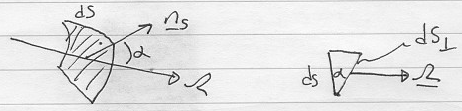
\includegraphics[height=1in]{DifferentialArea}
\end{center}
\end{figure}

Use the definition of $\vec{j} \rightarrow$ the expected number of particles crossing $dS$ along $\hat{e}_S$ with energy $[E, E + dE]$ and direction $[\vOmega, \vOmega + d\vOmega]$ at time $t$  
%
\[= \vec{j}(\vec{r}_s, E, \vOmega, t) \cdot d\vec{S} dE d\vOmega\]
%
Let $\vec{r}_s$ be a point on the surface and  $d\vec{S} = \hat{e}_S dS$.

Thus, the total leakage out of $V$ is
\[\Bigl[\int_S \vec{j}(\vec{r}_s, E, \vOmega, t) \cdot d\vec{S} \Bigr] dE d\vOmega \]

We can use divergence theorem to rewrite this w.r.t.\ $V$ (rather than $S$):
\[\int_S \hat{e}_S \cdot \vec{F} (\vec{r}) dS = \int_V \nabla \cdot \vec{F} (\vec{r}) dV\]
where
\[\nabla = \vec{i}\frac{d}{dx} + \vec{j}\frac{d}{dy} + \vec{k}\frac{d}{dz}\]
is the gradient operator.

This gives
\[\Bigl[\int_V d^3r \nabla \cdot \bigl( \underbrace{\vec{j}(\vec{r}_s, E, \vOmega, t)}_{\vec{v}n = v \vOmega n} \bigr) \Bigr] dE d\vOmega \]
%
And we can use this identity:
\begin{align}
%
\vOmega \cdot (\nabla f) &= \nabla \cdot \vOmega f \text{ because }\vOmega\text{ is not a function.} \\
\bigl[\nabla \cdot \vOmega f &= f(\underbrace{\nabla \cdot \vOmega}_{0}) + \vOmega \cdot (\nabla f)\bigr] \nonumber
\end{align}
%
\[ \boxed{\Bigl[\int_V d^3r \vOmega \cdot \nabla \bigl(v n(\vec{r}_s, E, \vOmega, t) \bigr) \Bigr] dE d\vOmega }\]

Note: $\vOmega \cdot \nabla$ represents the derivative along the direction of motion.

%--------------
\subsubsection{All Together Now}
The balance of neutrons: rate of change - production + loss = 0

Suppressing dependencies to save space for the moment
%
\begin{align}
\int_V d^3r \Bigl[\frac{\partial n}{\partial t} &- 
\int_{4\pi} d\vOmega' \int_0^{\infty} dE' \Sigma_s(E', \vOmega' \rightarrow E, \vOmega) v' n' \nonumber\\&-
\frac{\chi(E)}{4\pi} \int_{4\pi} d\vOmega' \int_0^{\infty} dE' \nu(E') \Sigma_f(E') v' n' -
s +
\Sigma_t v n + 
\vOmega \cdot \nabla v n \Bigr] = 0
\end{align}

We note that since the volume was arbitrarily chosen, the integral will only vanish if the integrand is zero 
\[\int_{\text{any }V} d^3r f(\vec{r}) = 0 \rightarrow f(\vec{r}) = 0 \:.\]

Now we have a balance relation that we can rearrange, and substitute in $\psi(\vec{r}, E, \vOmega, t) = vn(\vec{r}, E, \vOmega, t)$ to get what we usually call the Boltzmann Equation for neutron transport
%
\begin{align}
\frac{1}{v}\frac{\partial \psi(\vec{r}, E, \vOmega, t)}{\partial t} &+ 
\vOmega \cdot \nabla \psi(\vec{r}, E, \vOmega, t) +
\Sigma_t \psi(\vec{r}, E, \vOmega, t) = \nonumber\\
%
& \int_{4\pi} d\vOmega' \int_0^{\infty} dE' \Sigma_s(E', \vOmega' \rightarrow E, \vOmega) \psi(\vec{r}, E', \vOmega', t)  +\nonumber\\
%
& \frac{\chi(E)}{4\pi} \int_0^{\infty} dE' \nu(E') \Sigma_f(E') \int_{4\pi} d\vOmega' \psi(\vec{r}, E', \vOmega', t) +
s(\vec{r}, E, \vOmega, t)
\end{align}

%--------------
\subsubsection{Initial and Boundary Conditions}
\begin{enumerate}
\item \underline{Initial Condition}: We start with some initial ``known" state:
\[\psi(\vec{r}, E, \vOmega, 0) = \psi_0(\vec{r}, E, \vOmega)\]
for the problem domain. Note, the initial flux can be a functional expression.

\item \underline{Interface Condition}: the angular flux must be continuous along $\vOmega$ at all points, including material interfaces.

\begin{minipage}{0.5\textwidth}
\begin{figure}[H]
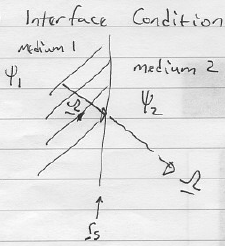
\includegraphics[height=2in]{InterfaceCondition}
%\caption{\label{fig:interfaceCondition} Interface Condition}
\end{figure}
\end{minipage} \hfill
\begin{minipage}{0.45\textwidth}
$\psi_1(\vec{r}_S, E, \vOmega, t) = \psi_2(\vec{r}_S, E, \vOmega, t)$\\ $\forall E$ and $\vOmega$.
\end{minipage}

\item \underline{Fixed Condition}: you can specify incoming flux

\begin{minipage}{0.45\textwidth}
\begin{figure}[H]
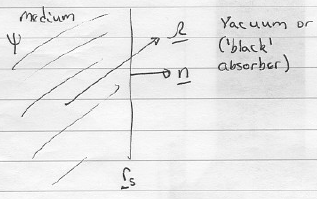
\includegraphics[height=1.75in]{FreeSurfaceCondition}
%\caption{\label{fig:FixedCondition} Fixed Condition}
\end{figure}
\end{minipage} \hfill
\begin{minipage}{0.5\textwidth}
$\psi(\vec{r}_S, E, \vOmega, t) = \psi_{IN}(\vec{r}_S, E, \vOmega, t)$ for $\vec{e} \cdot \vOmega < 0$: specifying incoming neutrons. Note, the incoming flux can be a functional expression; it can also be zero.

This is also equivalent to specifying the incoming partial current, $$\vec{j}^-(\vec{r}_S, E, t) = \int_{\vec{e} \cdot \vOmega < 0} d\vOmega (\vec{e} \cdot \vOmega) \psi(\vec{r}_S, E, \vOmega, t)$$.
\end{minipage}

\item \underline{Reflective Condition}: there is mirror symmetry at some surface:
\[\psi(\vOmega_{IN}) = \psi(\vOmega_{OUT})\]

\item \underline{Periodic Condition}: you know there is a repetition in the system
\[\psi(\vec{r}_S, E, \vOmega, t) = \psi(\vec{r}_S \pm \vec{p}, E, \vOmega, t)\]

\item \underline{Finiteness Condition}: to by physically valid we need to meet the condition $0 < \psi(\vec{r}_S, E, \vOmega, t) < \infty$, with the possible exception of point sources,

\item which we handle with the \underline{Source Condition}: localized sources are introduced as mathematical singularities at the location of the source.

For a source $s(\vec{r}_0, E, \vOmega, t)$:
\begin{align}
&\lim_{\vec{r} \rightarrow \vec{r}_0} \int_S dS \vec{e} \cdot \vOmega \psi(\vec{r}, E, \vOmega, t) = s(\vec{r}_0, E, \vOmega, t) \\
&s(\vec{r}, E, \vOmega, t) = s(\vec{r}_0, E, \vOmega, t)\delta(\vec{r} - \vec{r}_0)
\end{align}
\end{enumerate}


%---------------------------------------------
%---------------------------------------------
\subsection{Simplified Forms}

\subsubsection{One Speed}
Assume all particles are at the same speed, so we no longer need energy dependence.

%We assume all particles have the same speed, $\vec{v} = v_0 \cdot \vOmega$. Thus
%%
%\begin{align}
%n(\vec{r}, v, \vOmega, t) &= n(\vec{r}, \vOmega, t) \delta(v - v_0) \\
%\Sigma_s(\underbrace{E' \rightarrow E, \vOmega' \cdot \vOmega}_{\text{another way to write this}}) &= \Sigma_s(E,\vOmega' \cdot \vOmega)\delta(E' - E)
%\end{align}
%
% remove E integration and E dependence

\begin{align}
\frac{1}{v}\frac{\partial \psi(\vec{r}, \vOmega, t)}{\partial t} &+ 
\vOmega \cdot \nabla \psi(\vec{r}, \vOmega, t) +
\Sigma_t \psi(\vec{r}, \vOmega, t) = \nonumber\\
%
& \int_{4\pi} d\vOmega' \Sigma_s(\vOmega' \cdot \vOmega) \psi(\vec{r}, \vOmega', t)  
+ \frac{\nu \Sigma_f}{4\pi} \int_{4\pi} d\vOmega' \psi(\vec{r},  \vOmega', t) 
+ s(\vec{r}, \vOmega, t) 
%Q(\vec{r}, \vOmega, t)
\end{align}
%
%Where:
%\begin{align}
%Q(\vec{r}, \vOmega, t) &= \frac{1}{4\pi} \nu \Sigma_f \int_{4\pi} d\vOmega' \psi(\vec{r},  \vOmega, t) + S(\vec{r}, \vOmega, t) \\
%&= \frac{1}{4\pi} \bigl( \nu \Sigma_f \phi(\vec{r}, t) + s(\vec{r}, t) \bigr)
%\end{align}



%---------------------------------------------
\subsubsection{One Speed, One Dimensional}

We'd like to simplify even farther by only worrying about one dimension, so we'll get rid of $y$ and $z$.

\begin{minipage}{0.5\textwidth}
$\vec{r} = (x, y, z)$

$d\vOmega = \sin(\theta) d\theta	d\varphi = d\mu d\varphi$

Note $\mu = \cos(\theta)$ so $d\mu = \sin(\theta)$

$\Omega_x = \cos(\theta) = \mu$
\end{minipage} \hfill
\begin{minipage}{0.45\textwidth}
\begin{figure}[H]
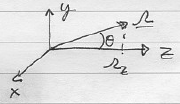
\includegraphics[height=1in]{1Dspace}
\caption{swap z for y, y for x, and x for z}
\end{figure}
\end{minipage}

% \vec{r} switched to x
\begin{align}
\frac{1}{v}\frac{\partial \psi(x, \vOmega, t)}{\partial t} &+ 
\bigl(\Omega_x \frac{\partial}{\partial x} + \cancel{\Omega_y \frac{\partial}{\partial y}} + \cancel{\Omega_z \frac{\partial}{\partial z}} \bigr)\psi(x, \vOmega, t) +
\Sigma_t \psi(x, \vOmega, t) = \nonumber\\
%
& \int_{4\pi} d\vOmega' \Sigma_s(\vOmega' \cdot \vOmega) \psi(x, \vOmega', t)  + 
\frac{\nu \Sigma_f}{4\pi} \int_{4\pi} d\vOmega' \psi(x,  \vOmega', t) + s(x, \vOmega, t)%+ Q(x, \vOmega, t)
\end{align}


%\begin{minipage}{0.3\textwidth}
%\begin{figure}[H]
%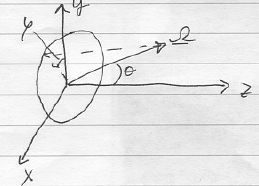
\includegraphics[height=1.5in]{AzimuthalSymmetry}
%%\caption{\label{fig:FixedCondition} Fixed Condition}
%\end{figure}
%\end{minipage} \hfill
%\begin{minipage}{0.65\textwidth}
%
%\end{minipage}
%
%Using this idea we can write things more cleanly:
%%
%% switch to just \mu
%\begin{align}
%\frac{1}{v_0}\frac{\partial \psi(x, \vOmega, t)}{\partial t} &+ 
%\mu \frac{\partial}{\partial x}\psi(x, \vOmega, t) +
%\Sigma_t \psi(x, \vOmega, t) = \nonumber\\
%%
%& \int_0^{2\pi} d\phi \int_{4\pi} d\vOmega' \Sigma_s(\vOmega' \cdot \vOmega) \frac{\psi(x, \mu', t)}{2\pi}  + 
%\frac{1}{4\pi} \nu \Sigma_f \int_0^{2\pi} d\phi \psi(x, \mu, t) + s(x, \mu, t)% 2\pi Q(x, \mu, t)
%\end{align}
%
%If \textbf{scattering is also isotropic}:
%\[\Sigma_s(\vOmega' \cdot \vOmega) = \frac{\Sigma_s}{4\pi} \]
%
%And we get the 1-group, 1-D, isotropic neutron TE:
%%
%% scattering is now iso, add in sources
%\begin{align}
%\frac{1}{v_0}\frac{\partial \psi(x, \mu, t)}{\partial t} &+ 
%\mu \frac{\partial}{\partial x}\psi(x, \mu, t) +
%\Sigma_t \psi(x, \mu, t) = \nonumber\\
%%
%& \frac{1}{2} \Sigma_s \int_{-1}^{1} d\mu' \psi(x, \mu', t)  
%+  \frac{1}{2} \bigl( \nu \Sigma_f \phi(x, t) + S(x, t) \bigr)
%\end{align}
%
%%---------------------------------------------
%\subsubsection{Steady State}
%If we get rid of time dependence.
%%
%\begin{equation}
%\mu \frac{\partial}{\partial x}\psi(x, \mu) +
%\Sigma_t \psi(x, \mu) = \frac{1}{2} \Sigma_s \int_{-1}^{1} d\mu' \psi(x, \mu')  
%+  \frac{1}{2} \bigl( \nu \Sigma_f \phi(x) + S(x) \bigr)
%\end{equation}
%
%
%And very finally - we can have the unrealistic case of \textbf{purely absorbing media}:
%%
%\begin{equation}
%\mu \frac{\partial}{\partial x}\psi(x, \mu) +
%\Sigma_a \psi(x, \mu) = \frac{1}{2} \bigl( \nu \Sigma_f \phi(x) + S(x) \bigr)
%\end{equation}


%--------------------------------------------
%--------------------------------------------
%--------------------------------------------
\section{Diffusion Equation Derivation}

We will now derive the diffusion equation by assuming the \textbf{angular flux depends only weakly on direction}, $\vOmega$. 
%
% Why?
Why derive the diffusion equation from the transport equation?
\begin{itemize}
\item Nuclear reactions and thus interaction rates only depend on the scalar flux
\item the angular flux lives in 7-D space (3 space, 2 angle, 1 energy, and 1 time)
\item the diffusion equation reduces this to 5-D space (3 space, 1 energy, and 1 time)
\end{itemize}

The diffusion equation is derived by starting with the transport equation and \textbf{integrating over all angles}. We'll use the \underline{one-group} version for simplicity, but this assumption is not needed for the derivation. 

Recall the definition of scalar flux and net current:
\begin{align}
\phi(\vec{r}, t) &= \int_{4\pi} d\vOmega \psi(\vec{r}, \vOmega, t) \\
\vec{J}(\vec{r}, t) &= \int_{4\pi} d\vOmega \vOmega \psi(\vec{r}, \vOmega, t)
\end{align}

%----------------------------
\subsection{Neutron Continuity Equation}
Now let's do the integration and go through it term by term (number the terms):
%
\begin{align}
\int_{4\pi} d\vOmega &\biggl[\frac{1}{v}\frac{\partial \psi(\vec{r}, \vOmega, t)}{\partial t} + 
\vOmega \cdot \nabla \psi(\vec{r}, \vOmega, t) +
\Sigma_t \psi(\vec{r}, \vOmega, t) = \nonumber\\
%
&\int_{4\pi} d\vOmega' \Sigma_s(\vOmega' \cdot \vOmega) \psi(\vec{r}, \vOmega', t)  
+ \frac{\nu \Sigma_f}{4\pi} \int_{4\pi} d\vOmega' \psi(\vec{r},  \vOmega', t)
+ s(\vec{r}, \vOmega, t)\biggr]
\end{align}
%
This is called the zeroeth order moment w.r.t $\vOmega$. 

\textbf{1.} No approximations
\begin{equation}
\frac{1}{v}\frac{\partial}{\partial t} \int_{4\pi} d\vOmega  \psi(\vec{r}, \vOmega, t) = \boxed{\frac{1}{v}\frac{\partial}{\partial t}\phi(\vec{r}, t)}
\end{equation}
%%%%
\textbf{3.} No approximations
\begin{equation}
\Sigma_t \int_{4\pi} d\vOmega \psi(\vec{r}, \vOmega, t) = \boxed{\Sigma_t \phi(\vec{r}, t)}
\end{equation}
%%%%
\textbf{5.} No approximations; but we will make use of the identity
\[\int_{4\pi} d\vOmega = \int_0^{\pi} \sin(\theta) d\theta \int_0^{2\pi} d\varphi = 4\pi \]
Thus
\begin{align}
\int_{4\pi} d\vOmega \frac{\nu \Sigma_f}{4\pi} &\int_{4\pi} d\vOmega' \psi(\vec{r},\vOmega', t) = \\
& 4\pi \frac{\nu \Sigma_f}{4\pi} \int_{4\pi} d\vOmega' \psi(\vec{r},\vOmega', t) = \boxed{\nu \Sigma_f \phi(\vec{r}, t)}
\end{align}

%%%%
\textbf{6.} No approximations
\begin{equation}
\int_{4\pi} d\vOmega s(\vec{r}, \vOmega, t) \equiv \boxed{S(\vec{r}, t)}
\end{equation}
%%%%
\textbf{4.} Further investigate the scattering cross section

Let's interchange the order of integrations over $\vOmega$ and $\vOmega'$:
%
\begin{align}
\int_{4\pi} d\vOmega &\int_{4\pi} d\vOmega' \Sigma_s(\vOmega' \cdot \vOmega) \psi(\vec{r}, \vOmega', t)\\
%
&= \int_{4\pi} d\vOmega' \bigl[ \int_{4\pi} d\vOmega \Sigma_s(\vOmega' \cdot \vOmega)\bigr] \psi(\vec{r}, \vOmega', t)
\end{align}

Then we can simplify the scattering term with this assumption (which is often true) that $\Sigma_s(\vOmega' \cdot \vOmega)$ is \textbf{azimuthally symmetric}, meaning it only depends on the angle of the scattering cosine $\mu =\vOmega' \cdot \vOmega$.  This implies
\[\int_{4\pi} d\vOmega \Sigma_s(\vOmega' \cdot \vOmega) = 2\pi \int_{-1}^{1} d\mu \Sigma_s(\mu) = \Sigma_s\]
%
And therefore:
%
\begin{align}
\text{scatterig integral }&= \Sigma_s \int_{4\pi} d\vOmega' \psi(\vec{r}, \vOmega', t) \\
%
&= \boxed{\Sigma_s \phi(\vec{r}, t)}
\end{align}
%%%%%%%
\textbf{2.} Finally, now we get to the trouble term: streaming
%
\[\int_{4\pi} d\vOmega \vOmega \cdot \nabla \psi(\vec{r}, \vOmega, t) = \nabla \cdot \int_{4\pi} d\vOmega \vOmega \psi(\vec{r}, \vOmega, t) = \nabla \cdot \vec{J}(\vec{r}, t) \]

\vspace*{2em}
When we put all of the terms together we get the \textbf{neutron continuity equation}. You can see that we have 1 equation, but 2 unknowns (technically 4 unknowns b/c $\vec{J}$ has 3 spatial components)
\begin{equation}
\frac{1}{v}\frac{\partial}{\partial t}\phi(\vec{r}, t) + 
\nabla \cdot \vec{J}(\vec{r}, t) + 
\Sigma_t \phi(\vec{r}, t) =
\Sigma_s \phi(\vec{r}, t) +
\nu \Sigma_f \phi(\vec{r}, t) +
S(\vec{r}, t)
\end{equation}

We at least have a relationship between $\phi$ and $\vec{J}$.

%-------------------------------------------
\subsection{First Angular Moment}

The next step is to take the first angular moment of the transport equation to try to develop additional relationships that we can use to solve for $\phi$. Thus, we multiply the one-group TE by $\vOmega$ and integrate over angle (with the zeroth moment we didn't do the multiplication first). 

NOTE: at this point I'm dropping the fission term for simplicity (the extension is straightforward). We will assume any fission neutrons are included in our source term, $S$. 


% Identities
We will use the following identities in this part of the derivation:
\begin{align} 
\int_{4\pi} d\vOmega \:\vOmega &= 0 \qquad \text{because }\vOmega\text{ is an odd function} \\
%
\int_{4\pi} d\vOmega\: \vOmega \vOmega &= \frac{4\pi}{3}\bar{\bar{I}} \qquad \bar{\bar{I}}\text{ is the identity tensor, which means} \\
%
&\int_{4\pi} d\vOmega\: \vOmega_i \vOmega_j = 0 \qquad i \neq j \nonumber \\
&\qquad \qquad = \frac{4\pi}{3} \qquad i = j \nonumber \\
%
\int_{4\pi} d\vOmega \: \vOmega \vOmega \vOmega &= 0 \qquad \\
\end{align}
%We are going to note that $\vOmega$ is a vector:
%\[\vOmega = \hat{e}_x \underbrace{\sin(\theta) \cos(\varphi)}_{\Omega_x} 
%+ \hat{e}_y \underbrace{\sin(\theta) \sin(\varphi)}_{\vOmega_y}
%+ \hat{e}_z \underbrace{\cos(\theta)}_{\vOmega_z} \]
%
%We will multiply the TE by each component separately to make things a little easier for ourselves. Looking first at $\Omega_x$ 
Multiplying by $\vOmega$ and dropping dependencies when appropriate:
%
\begin{align}
\int_{4\pi} d\vOmega\: \vOmega \frac{1}{v}\frac{\partial \psi}{\partial t} &+ 
\int_{4\pi} d\vOmega\: \vOmega \vOmega \cdot \nabla \psi + 
\int_{4\pi} d\vOmega\: \vOmega \Sigma_t \psi =\nonumber \\
&\int_{4\pi} d\vOmega\: \vOmega \int_{4\pi} d\vOmega'\: \Sigma_s(\vOmega' \cdot \vOmega) \psi(\vec{r}, \vOmega', t) +
\int_{4\pi} d\vOmega\: \vOmega s(\vec{r}, \vOmega, t)
\end{align}

Now we can go through term by term, just like how we got the continuity equation.

\textbf{1.}
\begin{equation}
\frac{1}{v}\frac{\partial}{\partial t} \int_{4\pi} d\vOmega\: \vOmega \psi(\vec{r}, \vOmega, t) = \boxed{\frac{1}{v}\frac{\partial \vec{J}}{\partial t}}
\end{equation}
%%%%
\textbf{3.} 
\begin{equation}
\Sigma_t \int_{4\pi} d\vOmega\: \vOmega \psi(\vec{r}, \vOmega, t) = \boxed{\Sigma_t  \vec{J}(\vec{r}, t)}
\end{equation}
%%%%
\textbf{5.} (was 6)
\begin{equation}
\int_{4\pi} d\vOmega\: \vOmega s(\vec{r}, \vOmega, t) \equiv \boxed{S_{1}(\vec{r}, t)}
\end{equation}
This is the first angular moment of the source term. 

%%%%
\textbf{4.} 

%First, we're flipping the prime order again inside the integral:
%\[\int_{4\pi} d\vOmega' \int_{4\pi} d\vOmega \Omega_x \Sigma_s(\vOmega' \cdot \vOmega) \psi(\vec{r}, \vOmega, t)\]

%We'll use the fact that $\vOmega$ is a unit vector and thus $\vOmega \cdot \vOmega = 1$. We're going to add this into our equation:
%\[ \int_{4\pi} d\vOmega' \bigl[\int_{4\pi} d\vOmega \Omega_x \vOmega \Sigma_s(\vOmega' \cdot \vOmega) \bigr] \cdot \vOmega \psi(\vec{r}, \vOmega, t) \]
%
%Next, recall that $\Sigma_s(\vOmega' \cdot \vOmega)$ depends only on $\mu_0 = \vOmega' \cdot \vOmega$:
%
%\[ 3 \int_{4\pi} d\vOmega' \bigl[\int_{4\pi} d\vOmega \Omega_x \Omega_x' \Sigma_s(\vOmega' \cdot \vOmega) \bigr] \cdot \Omega_x' \psi(\vec{r}, \vOmega, t) \]

For the scattering term we will do some mathematical manipulation. There are several ways to do this, but this one makes the most sense to me (different from Duderstadt and Hamilton).

Expand the scattering cross section in Legendre Polynomials, which are a sequence of orthogonal polynomials:
%
\[P_n(x) = \frac{1}{2^n n!}\frac{d^n}{dx^n} \bigl[\bigl( x^2 -1 \bigr)^n\bigr] \]

Then:
\begin{align}
\Sigma_s(\vOmega' \cdot \vOmega) &= \sum_{l=0}^{\infty} \frac{2l+1}{4\pi} \Sigma_{sl} P_l(\vOmega')P_l(\vOmega) \\
%
\Sigma_s(\vOmega' \cdot \vOmega) &=  \frac{1}{4\pi}\Sigma_{s0} \qquad l=0 \text{ isotropic} \\
& \text{note } P_0 (\vOmega) = 1 \\
%
\Sigma_s(\vOmega' \cdot \vOmega) &=  \frac{1}{4\pi}\bigl( \Sigma_{s0} + 3\vOmega' \vOmega \Sigma_{s1} \bigr) \qquad l=1 \text{ linearly isotropic}\\
& \text{note } P_1 (\vOmega) = \vOmega 
\end{align}

We're going to \textbf{assume that scattering is at most linearly anisotropic}, so we will stop expanding here.

Substitute the $l=1$ linearly anisotropic truncation into the equation and use some of our identities:
%
\begin{align}
\frac{1}{4\pi} \int_{4\pi}  \vOmega &d\vOmega \int_{4\pi} d\vOmega' \bigl[\Sigma_{s0} + 3\vOmega' \vOmega \Sigma_{s1} \bigr] \psi(\vec{r}, \vOmega', t) = \nonumber\\
%
& \underbrace{\frac{1}{4\pi} \int_{4\pi} d\vOmega \vOmega}_{0}  \underbrace{\int_{4\pi} d\vOmega'\:  \Sigma_{s0}\psi(\vec{r}, \vOmega', t)}_{\Sigma_{s0} \phi(\vec{r},t)} +
%
\frac{1}{4\pi} \underbrace{\int_{4\pi} d\vOmega \:\vOmega \vOmega}_{4\pi/3 \bar{\bar{I}}} \underbrace{\int_{4\pi} d\vOmega'\: \vOmega' 3  \Sigma_{s1}\psi(\vec{r}, \vOmega', t)}_{3\Sigma_{s1} \vec{J}(\vec{r},t)} \\
%
&= \boxed{\Sigma_{s1} \vec{J}(\vec{r},t)}
\end{align}
%%%%%%%%
\textbf{2.} And once again, the trouble term: streaming
%
\[\int_{4\pi} d\vOmega \vOmega \vOmega \cdot \nabla \psi(\vec{r}, \vOmega, t) = \nabla \cdot \int_{4\pi} d\vOmega \vOmega \vOmega \psi(\vec{r}, \vOmega, t) \]

\vspace*{2em}
All together this is the \textbf{current continuity equation}:
\begin{equation}
\frac{1}{v}\frac{\partial \vec{J}}{\partial t} 
+ \nabla \cdot \int_{4\pi} d\vOmega \vOmega \vOmega \psi(\vec{r}, \vOmega, t) +
\Sigma_t  \vec{J}(\vec{r}, t) =
\Sigma_{s1} \vec{J}(\vec{r},t)
+ S_{1}(\vec{r}, t) 
\label{eq:current1}
\end{equation}

Now we have two moment equations that give us 4 total equations (neutron continuity and 3 tensor equations) and 10 unknowns ($\phi$, 3 from the $\vec{J}$, and 6 from the new tensor term). 

Taking higher moments by repeating the multiply by $\vOmega$ and integrating isn't going to help matters.


%-----------------------
%-----------------------
\subsection{Linearly Anisotropic Approximation}
And finally, \underline{we introduce an approximation about the angular flux} (so far we have only approximated the scattering as linearly anisotropic). We now \textbf{assume that the angular flux is at most linearly anisotropic} as well.

To implement this assumption, the angular flux is expanded in angle and only the first two terms are retained:  
%
\begin{align}
\psi(\vOmega) &=  \frac{1}{4\pi}\bigl( \psi_{0} + 3\vOmega \cdot \vec{\psi_{1}} \bigr) \qquad l=1 \text{ linearly isotropic} \\
%
\psi(\vOmega) &\cong \frac{1}{4\pi}\bigl(\phi(\vec{r}, t) + 3 \vOmega \cdot \vec{J}(\vec{r}, t)\bigr) \:.
  \label{eq:angExpand} 
\end{align}
The truncated angular flux expansion is then inserted into the streaming term in Equation \eqref{eq:current1}, giving 
%
\begin{align}
  \nabla \cdot \frac{1}{4\pi} \int d \vOmega \:\vOmega \vOmega  \bigl(\phi(\vec{r}, t) + 3 \vOmega \cdot \vec{J}(\vec{r}, t)\bigr) &=  
%
\nabla \cdot \frac{1}{4\pi} \bigl[\int d \vOmega \:\vOmega \vOmega  \phi(\vec{r}, t) 
%
+ 3 \underbrace{\int d \vOmega \:\vOmega \vOmega \vOmega \cdot \vec{J}(\vec{r}, t)}_{0} \bigr] \nonumber \\
% 
&= \nabla \cdot \frac{1}{4\pi} \frac{4\pi}{3}\bar{\bar{I}} \phi(\vec{r}, t) \\
%
  &= \frac{1}{3} \nabla \phi(\vec{r}, t) 
  \label{eq:firstTerm}
\end{align}

With this approximation, the current continuity equation becomes:
\begin{equation}
\frac{1}{v}\frac{\partial \vec{J}}{\partial t} 
+ \frac{1}{3} \nabla \phi(\vec{r}, t) +
\Sigma_t  \vec{J}(\vec{r}, t) =
\Sigma_{s1} \vec{J}(\vec{r},t)
+ S_{1}(\vec{r}, t) 
\label{eq:current1}
\end{equation}
%
Next we'll define:
\begin{align}
\Sigma_a &\equiv \Sigma_t - \Sigma_{s0} \qquad \text{``absorption" cross section}\\
\Sigma_{tr} &\equiv \Sigma_t - \Sigma_{s1} \qquad \text{``transport" cross section}
\end{align}

Let's substitute these into our equation set:
%
\begin{align}
\frac{1}{v}\frac{\partial}{\partial t}\phi(\vec{r}, t) + 
\nabla \cdot \vec{J}(\vec{r}, t) + 
\Sigma_a \phi(\vec{r}, t) =
\nu \Sigma_f \phi(\vec{r}, t) +
S(\vec{r}, t) \\
%
\frac{1}{v}\frac{\partial \vec{J}}{\partial t} 
+ \frac{1}{3} \nabla \phi(\vec{r}, t) +
\Sigma_{tr}  \vec{J}(\vec{r}, t) =
S_{1}(\vec{r}, t) 
\end{align}
%
These are the $P_1$ equations because they are derived from the 0th and 1st Legendre polynomial expansion of the angular flux. And we now have 4 equations with 4 unknowns!

\subsubsection{Fick's Law}
If we also assume \underline{steady state} (or weak temporal dependence) and \underline{an isotropic source}, the current continuity equation becomes
%
\begin{align}
\frac{1}{3} \nabla \phi(\vec{r}, t) +
\Sigma_{tr}  &\vec{J}(\vec{r}) = 0 \\
&\boxed{\vec{J}(\vec{r}) = -\frac{1}{3\Sigma_{tr}} \nabla \phi(\vec{r}, t) = -D\nabla \phi(\vec{r}, t) } \qquad \text{Fick's Law}
\end{align}
%
where
\[D = \frac{1}{3\Macro_{tr}} = \frac{1}{3(\Macro_t(\vec{r}) - \Macro_{s1}(\vec{r}))}\] 
is the diffusion coefficient. 

 ---------------------------------------\\
\textbf{Aside:} $\Macro_{s1}  = \int d\vOmega \:\vOmega \Macro_{s}$. When we include the azimuthally symmetric assumption we get $\Macro_{s1} = \bar{\mu}_{0}\Macro_{s}$, where $\bar{\mu}_{0}$ is the average cosine of the scattering angle.

For elastic scattering from stationary nuclei when s-wave scattering is present in the center of mass frame, $\bar{\mu_{0}} = \frac{2}{3A}$ where $A$ is atomic mass number. 

With all of this, $\Sigma_{tr} = \Sigma_t - \bar{\mu}_0 \Sigma_s$.

%While we're dealing with the one group version of this, the derivation is technically only valid in one-speed. The reason is that to simplify common procedure to simplify the energy dependence is to \textbf{neglect the anisotropic contribution to energy transfer in a scattering collision}.
%
% Mathematically this means $\Macro_{s1}(E' \to E) = \Macro_{s1}(E) \delta(E' = E)$, giving $\int dE' \:\Macro_{s1}(\vec{r}, E' \to E)J(\vec{r},E') = \bar{\mu_{0}}\Macro_{s}(\vec{r},E)J(\vec{r},E)$.
 ---------------------------------------

\underline{Punchline:} Fick's Law gives us a clear relationship between current and scalar flux. Now we can write the diffusion equation in terms of only $\phi$!
%
\begin{equation}
\boxed{\frac{1}{v}\frac{\partial}{\partial t}\phi(\vec{r}, t) 
-\nabla \cdot D\nabla \phi(\vec{r}, t) + 
\Sigma_a \phi(\vec{r}, t) =
\nu \Sigma_f \phi(\vec{r}, t) +
S(\vec{r}, t)} \:.
\end{equation}

We can also re-write our angular flux expansion as
\[\psi(\vec{r}, \vOmega, t) \cong \frac{1}{4\pi}\Bigl(\phi(\vec{r}, t)  -\frac{1}{\Sigma_{tr}} \nabla \phi(\vec{r}, t)\Bigr) \:.\]

The physical interpretation of the diffusion process is that the ``flow" of neutrons is driven by a spatial gradient of flux. Or rather, neutrons diffuse from high to low concentration areas.

You can see the driving function in Fick's Law: 

Equilibrium is at any location where $\vec{J} = 0$: there are an equal number of neutrons crossing the interface in both directions. 

When we're not in equilibrium, more neutrons will be scatter from the side with larger $\phi$ to the side with lower $\phi$. Hence the net migration is opposed to the gradient (matching the negative sign). 

%-----------------------
%-----------------------
\subsection{Initial and Boundary Conditions}

We now need one initial condition and two boundary conditions. We will also use some other information.

\underline{Mean free path} is the mean distance from the last collision.
\[\lambda_{t} = \frac{1}{\Sigma_t} \qquad \lambda_{tr} = \frac{1}{\Sigma_{tr}}\]
%
If scattering is 
\begin{itemize}
\item isotropic, then $\bar{\mu}_0 = 0$ and $\lambda_{tr} = \lambda_{t}$
\item forward peaked, then $\bar{\mu}_0 > 0$ and $\lambda_{tr} > \lambda_{t}$
\end{itemize}	

\textbf{Initial conditions} are pretty easy:
\[\phi(\vec{r}, 0) = \phi_0(\vec{r}) \qquad \forall \vec{r} \in V \:.\]

\textbf{Basic requirements}: still need 
\begin{itemize}
\item the flux to be real and positive: $0 \leq \phi$
\item and bounded: $\phi < \infty$ except near mathematical approximations (the source condition). 
\end{itemize}

\subsubsection{Interface Conditions}
These are also fairly straightforward. We take the 0th and 1st moments of our TE condition
\[\psi_1(\vec{r}_S, \vOmega, t) = \psi_2(\vec{r}_S,\vOmega, t)\qquad \forall \vOmega\]
and we get two equations rather than one. Now
\begin{align}
\phi_1(\vec{r}, t) &= \phi_2(\vec{r}, t) \\
\vec{J}_1(\vec{r}, t) &= \vec{J}_2(\vec{r}, t)
\end{align}

\subsubsection{Vacuum Boundary Condition}
These aren't quite so simpley. We start by thinking about the transport non-reentrant condition: 
\[\psi(\vec{r}_s, \vOmega, t) = 0 \text{ for } \vOmega \cdot \hat{e}_s < 0 \:,\]
%
which is a mathematical statement that there are no neutrons entering our volume. Also written as
\[J_{-}(\vec{r},t) = \int_{\vOmega \cdot \hat{e}_s < 0} d\vOmega \: \vOmega \cdot \hat{e}_s \psi(\vec{r}_s, \vOmega, t) = 0 \:.\]

However, with diffusion theory
\[\psi(\vec{r}_s, \vOmega, t) \cong \frac{1}{4\pi}\bigl(\phi(\vec{r}_s, t)  -\frac{1}{\Sigma_{tr}} \nabla \phi(\vec{r}_s, t)\bigr)\]
%
and our partial currents become
%
\begin{align}
J_{\pm} &= \int_{2\pi^{\pm}} d\vOmega \: \vOmega \cdot \hat{e}_s \psi(\vec{r}_s, \vOmega, t) =\\
&\cong \frac{1}{4} \phi(\vec{r}, t) \mp \frac{D}{2} \hat{e}_s \cdot \nabla \phi(\vec{r}_s, t) = 0
\end{align} 
%
For a 1-D slab with vacuum boundary at $x=x_s$:
%
\begin{align}
J_{-}(\vec{r}_s, t) = J_{-}(x_s, t) &= \frac{1}{4} \phi(x_s, t) + \frac{D}{2}\frac{d \phi}{dx}\Bigm\lvert_{x_s} = 0 \\
\text{Or } \qquad \frac{1}{\phi(x_s, t)}\frac{d \phi}{dx}\Bigm\lvert_{x_s} &= -\frac{1}{2D}
\end{align}

This relationship implies that linearly extrapolating the flux beyond the vacuum boundary would lead to a vanishing flux at the point
\[\tilde{x}_s = x_s + 2D = x_s + \frac{2}{3}\lambda_{tr}\]
%
Thus, the vacuum condition $J_{-}(x_s) = 0$ is usually replaced with $\phi(\tilde{x}_s)= 0$. Additionally, computation with more detailed transport theory leads to an \textbf{extrapolation distance} of $0.7104\lambda_{tr} = z_0$ rather than $\frac{2}{3}\lambda_{tr}$.
%
\begin{figure}[h!]
\begin{center}
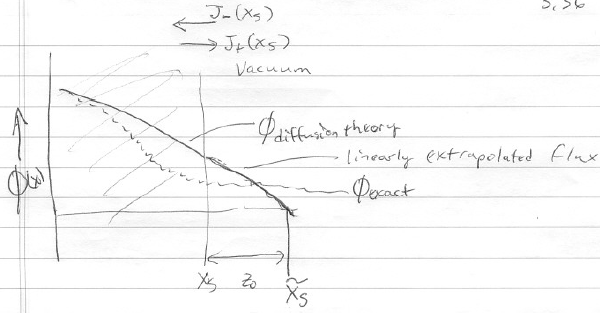
\includegraphics[height=3 in]{DiffusionBC}
\end{center}
\end{figure}

In reality, though, $\lambda_{tr} \sim 0$ [cm] compared to the size of a reactor core [m]. 


%------------------------------------------
\subsection{Helmholtz Form}

We can write the diffusion equation in steady state this way:
%
\begin{align}
-\nabla \cdot D\nabla \phi(\vec{r}) + 
\Sigma_a \phi(\vec{r}) &= Q(\vec{r}) \\
%
\text{Where }\qquad Q(\vec{r}) &=
\nu \Sigma_f \phi(\vec{r}) +
S(\vec{r})
\end{align}
%
which can be written as the Helmholtz equation of applied mathematics:
%http://en.wikipedia.org/wiki/Helmholtz_equation
%
\begin{align}
\nabla^2 \phi(\vec{r}) - \frac{1}{L^2}\phi(\vec{r}) &= \frac{-Q(\vec{r})}{D} \\
\text{Where }\qquad L &\equiv \frac{D}{\Sigma_a}
\end{align}
%
$L$ is called the neutron diffusion length. This is ``how far a neutron diffuses from a source prior to absorption". 

In the Helmholtz formulation $\phi$ is amplitude and $\frac{1}{L}$ is wave number. 

This formulation is useful because we know how to solve it. We write
\[\phi(\vec{r}) = \phi_H(\vec{r}) + \phi_P(\vec{r}) \:,\]

For example, we often have:
\[\phi_H(\vec{r}) = A\exp\bigl(-\frac{|\vec{r}|}{L}\bigr) + B\exp\bigl(-\frac{|\vec{r}|}{L}\bigr) \:.\]

Going through how to solve this analytically in a variety of circumstances, geometries, etc.\ is another class (NE 150/250). We're going to focus on numerical solution techniques. But first, one more thing.

%------------------------------------------
\subsection{Criticality Calculations}

We can write our DE in steady state for a nuclear reactor core:
%
\begin{align}
-\nabla \cdot D\nabla \phi(\vec{r}) + 
\Sigma_a \phi(\vec{r}) &= \nu \Sigma_f \phi(\vec{r}) \\
\text{with} \qquad \phi(\tilde{x}_s) &= 0
\end{align}
%
Unless we have the proper combination of core composition ($\Sigma_a$, $\Sigma_f$, $D$) and geometry ($\vec{r}$ ,$\vec{r}_s$), there is \underline{no} general solution. 

To deal with this, we introduce a parameter $k$ into the equation:
%
\begin{equation}
-\nabla \cdot D\nabla \phi(\vec{r}) + 
\Sigma_a \phi(\vec{r}) = \frac{1}{k}\nu \Sigma_f \phi(\vec{r})
\end{equation}
%
Then, for any value of $k$ we assert that there is always a solution. We use an iterative process to find the condition when $k=1$, called `critical'.

A reactor is called \textbf{``critical''} if the chain reaction is self-sustaining and time-independent. Another way to think of the addition of $k$ is to assume $\nu$ can be adjusted to obtain a time-independent solution by replacing it with $\frac{\nu}{k}$, where $k$ is the parameter expressing the deviation from critical. 

This substitution changes the transport equation into an \textbf{eigenvalue problem.} A spectrum of eigenvalues can be found, but at \textbf{long times only the non-negative solution corresponding to the largest real eigenvalue will dominate}, and that's $k$. 

$k$ can be thought of as the asymptotic ratio of the number of neutrons in one generation to the number in the next.

%--------------------------------------------------------------------
\bibliographystyle{plain}
\bibliography{15-19-te-de} 

\end{document}